\begin{figure}[ht]
\centering
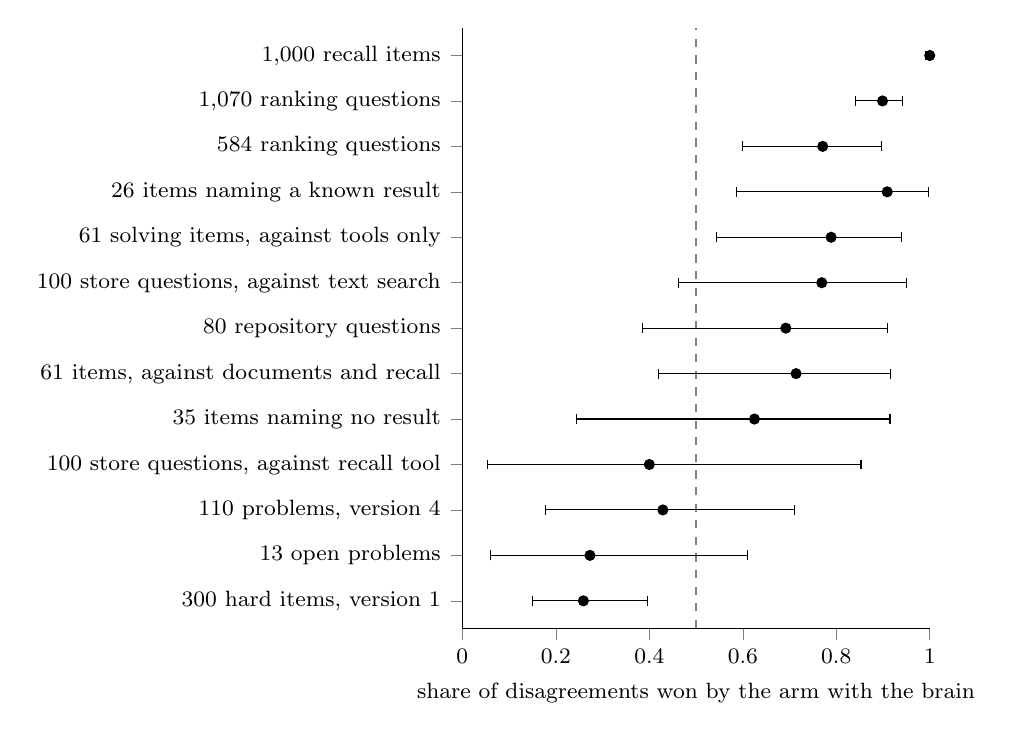
\begin{tikzpicture}
\begin{axis}[
  width=0.62\textwidth, height=9.2cm,
  xmin=0, xmax=1, ymin=0.4, ymax=13.6,
  xlabel={share of disagreements won by the arm with the brain},
  ytick={1,...,13},
  yticklabels={
    {300 hard items, version 1},
    {13 open problems},
    {110 problems, version 4},
    {100 store questions, against recall tool},
    {35 items naming no result},
    {61 items, against documents and recall},
    {80 repository questions},
    {100 store questions, against text search},
    {61 solving items, against tools only},
    {26 items naming a known result},
    {584 ranking questions},
    {1{,}070 ranking questions},
    {1{,}000 recall items}},
  yticklabel style={font=\footnotesize},
  xticklabel style={font=\footnotesize},
  xlabel style={font=\footnotesize},
  tick align=outside, axis x line*=bottom, axis y line*=left,
]
\addplot[gray, dashed] coordinates {(0.5,0.4) (0.5,13.6)};
\addplot[only marks, mark=*, mark size=1.8pt, black,
  error bars/.cd, x dir=both, x explicit]
  table[x=s, y=y, x error minus=m, x error plus=p] {
  y  s      m      p
  1  0.259  0.109  0.138
  2  0.273  0.213  0.337
  3  0.429  0.252  0.282
  4  0.400  0.347  0.453
  5  0.625  0.380  0.290
  6  0.714  0.295  0.202
  7  0.692  0.306  0.217
  8  0.769  0.307  0.181
  9  0.789  0.245  0.150
  10 0.909  0.322  0.089
  11 0.771  0.172  0.125
  12 0.899  0.057  0.042
  13 1.000  0.008  0.000
  };
\end{axis}
\end{tikzpicture}
\caption{The comparisons of the brain against a baseline on one scale: the share of the disagreeing items won by the arm with the brain, with an exact $95\%$ Clopper--Pearson interval. The dashed line is no effect. The four lowest rows are tests on which the brain did not help; the rows for versions~1 and~4 concern earlier versions on item sets and baselines of their own, and the open-problems row is a referee's pairwise preference. Intervals that cross the line are inconclusive, not evidence of equal accuracy.}
\label{fig:effects}
\end{figure}
